%SourceDoc ../YourName-Dissertation.tex
\chapter{Introduction -- Urban Computing} \label{chapter1:introduction}



With the advent of information age, more and more data are collected in the urban space. Using various urban data to solve real urban problem is called urban computing.



\section{The Opportunities from Urban Data}


In the urban space, more and more  data are available. Generally speaking, they have the following properties:

\textbf{Variety} refers to the heterogeneous data sources. As shown in Figure~\ref{fig:demo-data}, there is various types of data in the urban space. In the city, we can collect traffic data, Point-of-interest (POI), air quality measure, weather,  city noise complaints, and many more. Different types of data lead to different format in the data. For example, the air quality measure and weather is global over the city. Meanwhile, the crime incidents and taxi trip data have specific location information.


\textbf{Volume} of urban data is generally large. For example, there are more than $380,000$ POIs in New York City and $112,000$ POIs in Chicago. According to the Chicago public crime incidents record, there are over $5.8$ millions of records in the past 15 years. Each of the crime records have detailed information on the date, location, and crime description. 


\textbf{Velocity} refers to the speed that new data is generated, which is also huge in the urban space. For example, there are almost half million taxi trips are generated in New York City each day, and there are 621 millions of tweets posted each day.

These big data enable the opportunities to look into many urban problems, such as traffic anomaly detection,  travel time estimation, city noise diagnosing, from a new angle.


\begin{figure}[h]
\centering
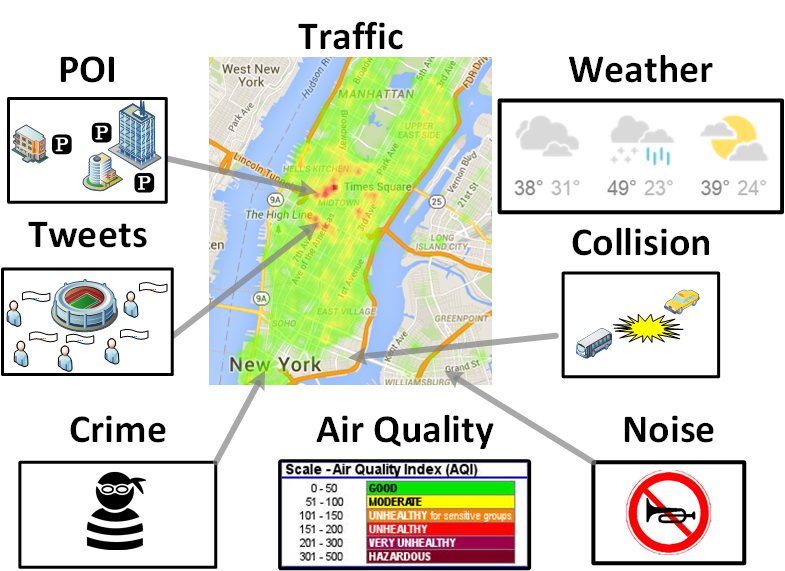
\includegraphics[width=0.9\textwidth]{fig/intro-data.png}
\caption{Use data collected in the urban space to address real urban problems.}
\label{fig:demo-data}
\end{figure}




\subsection{A New Type of Data: Mobility Flow}


As the advance to positioning technology, we are able to collect more and more mobility data.
In the urban space, the trajectories of massive public transportation vehicle are recorded at minute intervals; the taxi/urban trips are recorded by pickup/drop-off locations and time; personal trajectories are tracked by health related mobile App, people's home and office location are surveyed by US Census Bureau.


The mobility data is a new type of data, because it is not attached to one specific point as most of other urban data.
The mobility data tracks the movement of people among two or several locations. The ability to connect various locations make the mobility data unique and important~\cite{ZCWY14}.




\section{Model Interactions In Urban Space}

\emph{My research focus is to capture the complicated interactions in the urban space with the new flow data}. Consider the following one example.


\textbf{Example} \emph{Policy makers are deciding where to construct a shelter for families that are victims of violence. They understand the value of locating the shelter geographically far from violent neighborhoods. One possible choice is to locate the shelter in a neighborhood that is 10 miles from the violent neighborhoods where vulnerable families previously lived. However, a deeper analysis may reveal that the new neighborhood, though geographically removed from the old neighborhood, may still have strong social flows (connections caused by commutes, family visits) with the old neighborhood. Emerging research suggests that a great deal of crime happens in areas that are socially connected to offenders' neighborhoods. This suggests that shelters may benefit from being located in a neighborhood that is also socially isolated from violence (e.g., with weak communication and commuting interactions with the violent neighborhoods that shelter residents fled from) while socially connected to jobs, services, and resources.}


This example shows that measuring interactions of communities is an important problem to answer.


In the urban space, a model of \textbf{interactions} bring solutions to the several fundamental data mining questions. We propose to view the city as a spatial network of communities linked by ``hyperlink'' flow. The questions we can answer are
\begin{itemize}
\item Understand nodes using links. Estimate an unobserved property of focal community, given the observations on other communities and other types of data. For example, the crime rate in a residential neighborhood could be impacted by  non-adjacent but flow-connected neighborhoods, because the residents in the neighborhoods are also exposed to and influenced by the environment in the workplace.
\item Understand links using nodes. Are certain properties of two connected nodes associated with the type and volume of the flow connections? For example, given the crime profiles of two connected communities, which type of interactions (taxi, LEHD, or space continuity) is more important in forming the crime properties?
\item Identify the fundamental dependency structure among properties of nodes. For example, the crime rate of two connected communities may show a strong correlation. However, this does not necessarily mean that high crime rate in one community lead to the high crime in another. The crime is very likely to be caused by other properties. 
\end{itemize}




\subsection{Literature}


Traditionally, most urban research  do not use flow data, since the data is not available. For example, researchers have used demographic information (e.g., population poverty level, socioeconomic disadvantage, racial composition of population) to estimate the crime rate in a community~\cite{GrSa09}. However,  such demographic information only contains partial information about the neighborhoods and does not dynamically reflect the changes in the community. Using only demographic information will result in a relative error of at least 30\% for crime rate estimation in Chicago (refer to experiment section in the paper).



\textbf{Use spatial influence as interactions}.
Since there is no flow data available, spatial similarity is widely accepted assumption to model the region interactions. \textbf{Spatial similarity} assumes that spatially adjacent regions tend to have similar properties. In urban space, most data reflect the properties of human beings, such as the traffic volume, crime count, and geo-tagged tweets. Therefore, these data are attached to human crowd instead of a specific location. 
In the urban space, the intuition behind the \textbf{spatial similarity} is that human movement is regular, and most of our daily activities are conducted in a limited area.

There is one existing study using the geographical influence~\cite{Ans02} to estimate the crime rate, i.e., the crime in the nearby communities can be propagated to the focal community. But this geographical influence is of little help in improving the crime inference on top of demographic feature, with at most 0.4\% relative improvement in our experiments. This is probably because the nearby communities also share similar demographics, which limits the additional benefit of geographical influence. In the study, spatial autoregressive model is used

\begin{equation}
\label{eq:sar}
y = \rho_1 W^{spatial} y + X \beta + \epsilon,
\end{equation}
where $y$ is the crime count, $X$ is the demographics property, and $W^{spatial}$ is an $n\times n$ spatial distance matrix.



\textbf{Simple extension on spatial influence model}
It is easy to extend the spatial autoregressive model in Equation~\ref{eq:sar} with a social flow matrix.
\begin{equation}
\label{eq:sar2}
y = \rho_1 W^{spatial} y + \rho_2 W^{network} y + X \beta + \epsilon,
\end{equation}
where $W^{network}$ is an $n\times n$ social distance matrix.
It is clearly that the interaction term $\rho_2 W^{network} y$ is ad-hoc, since there could be other combinations like $\rho_3 W^{network} x_1$.





\subsection{Drawbacks}

\textbf{Define interaction is non-trivial}. There are too many possibilities in constructing interactions, and it is very ad-hoc as shown in Equation~\ref{eq:sar2}. The interaction among two regions involves the flow and some nodal properties. There are many different types of flow such as taxi flow, work-office flow, etc, each of which can take various formats, for example, used as raw flow or normalized by in/out flow. There are also many nodal properties that could interact with their neighbors, such as various demographics features. Above that there are all kinds of function that we can use to define interactions, such as multiplication or exponential. Therefore, the construction of interaction is totally ad-hoc. 


\textbf{The interaction could be spatial non-stationary}. The model in Equation~\ref{eq:sar2} is a global model, which assumes the statistic interaction does not vary over space. However, some urban data have spatial non-stationary property. Use Chicago crime as example, shown in Figure~\ref{fig:chi-crime}. It is clear that using global estimates of relationships can present misleading interpretations of local relationships.


\begin{figure}[h]
\centering
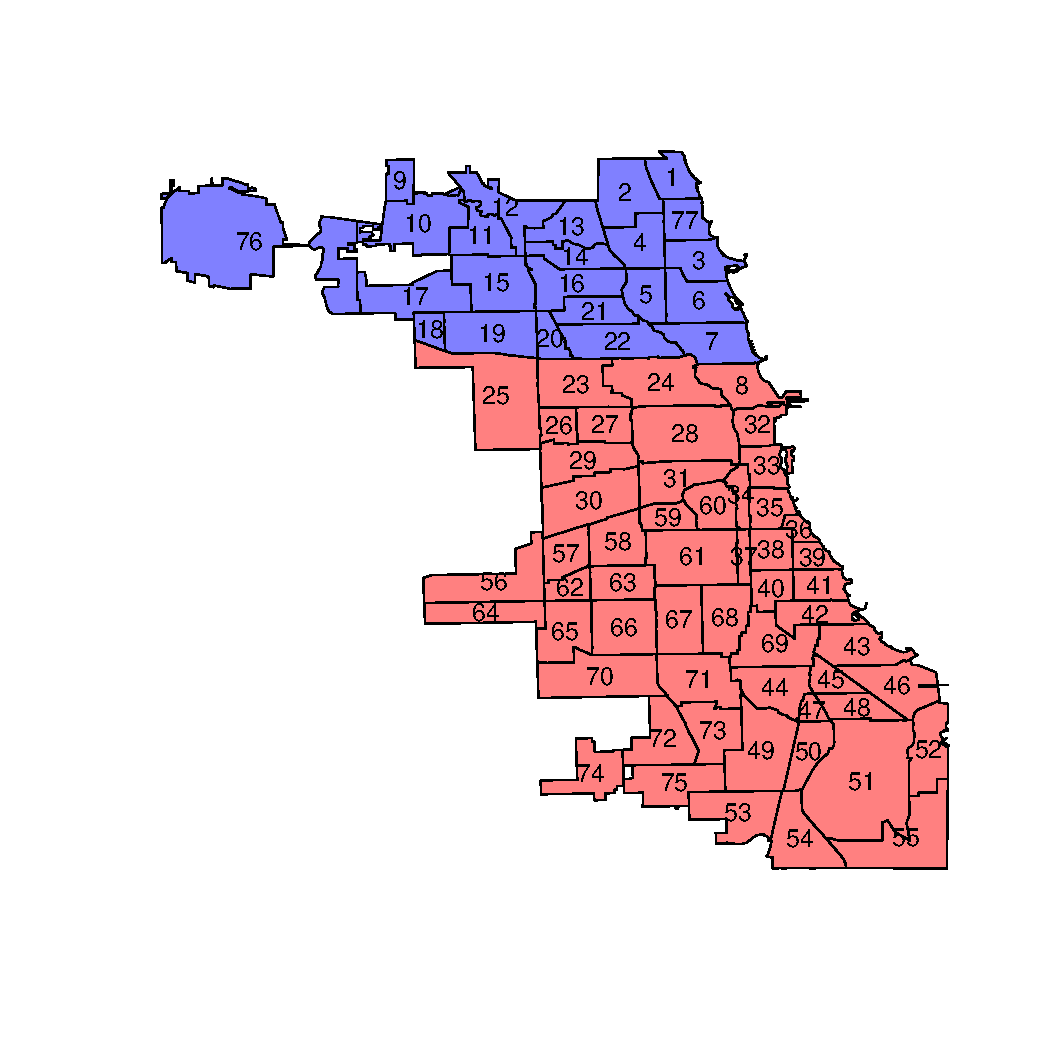
\includegraphics[width=0.45\textwidth]{fig/north-south-split.pdf}
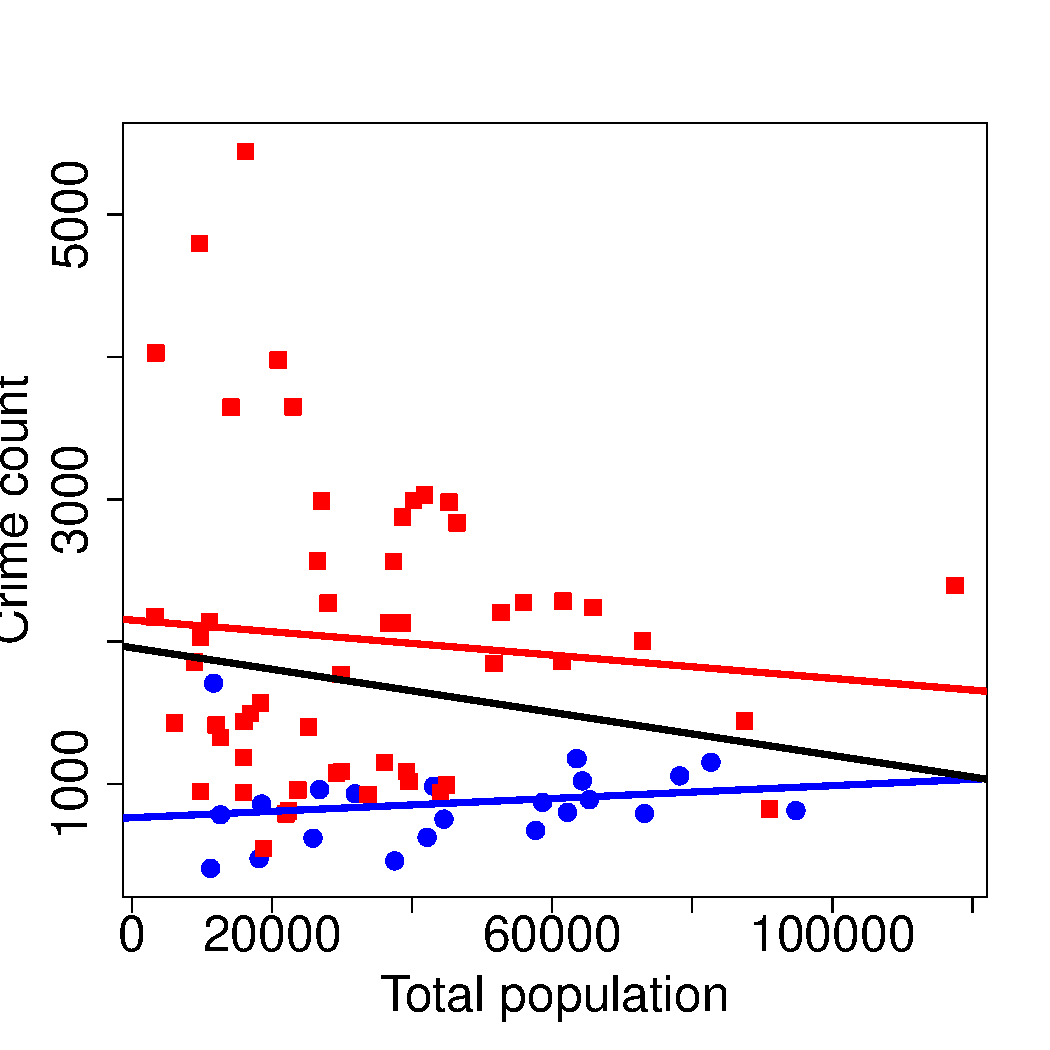
\includegraphics[width=0.45\textwidth]{fig/crime-pop.pdf}
\caption{The crime count vs. total population relationship shows spatial non-stationary property.}
\label{fig:chi-crime}
\end{figure}



\section{A Unified Graphical Model}

We propose a unified graphical model to capture the interactions among regions. Since various flow connect regions into various network. A graphical model is a natural way to represent the whole system. Additionally, this model can address the two drawbacks mentioned above.

To address the non-trivial definition of interaction. In the graphical model we model the interaction of two communities is a hidden variable. This hidden variable is connected with the observations on both flow and nodal properties. We can learn the interaction from the network.

To address the spatial non-stationarity. Each region is built as separate node in the graphical model. This way, the conditional probability 
\[ P(y_i | X_i) \]
is different at different regions, which is equivalent to have mutliple local models to capture the different relations between $y$ and $X$.





In next chapter we study the first problem - ``using links to understand nodes''. We use crime inference as an example, in which we use an enhanced spatial autoregressive model to predict crime count of a community using its neighbors. In Chapter \ref{ch:crf}. We first discuss the missing property of a spatial autoregressive model, which is the spatial non-stationarity. To address this, we propose a conditional random field based  graphical model. This model is superior than other method in the literature, such as geographically weighted regression. Finally, there is a research plan in Chapter \ref{ch:plan}.



